% Section content template for individual Educative lessons
% This file contains the actual content for a specific section
% Generated from Educative API section content

% Section: Use Case Diagram for LinkedIn
% Section ID: 6663591366492160
% Section Slug: use-case-diagram-for-linkedin
% Generated: 2025-12-14T13:34:19.223854

Let's build LinkedIn's use case diagram and understand the relationship between its different components. First , we'll define the different elements of our LinkedIn system, followed by the complete use case diagram.

\subsection{System}\label{DklM0cQ5mKO9iJUQZ3MRx}
\\
Our system is LinkedIn.

\subsection{Actors}\label{oSnFTfwG3rrOCuv6Nrpfo}
\\
Now, we'll define the main actors of LinkedIn.

\subsubsection{Primary actors}\label{n1JHUfylCqtYzkCQHBbON}

\begin{itemize}
\item
\protect\phantomsection\label{5RFkZE-ZCJAZnkj4FrXZB}
\textbf{User:} This actor can create a profile including their professional information. They can create posts, apply for jobs, follow pages, and join groups. They can also interact with other users by sending them connection invitations and messages, commenting on their posts, and so on.
\end{itemize}

\subsubsection{Secondary actors}\label{a1O8t-Eqp74zP-yCsssww}

\begin{itemize}
\item
\protect\phantomsection\label{i_AuWU5YGd5aXqfGPWzdB}
\textbf{System:} This sends notifications for new connection requests, messages, comments, posts, recommendations, and other relevant events.
\end{itemize}

\subsection{Use cases}\label{hh6mCh17hN-GtS1sKl7EU}
\\
In this section, we'll define LinkedIn's use cases. We have listed them in order of their respective interactions with a particular actor.
\begin{quote}
\textbf{Note:} Some use cases will occur multiple times because they are shared among different actors in the system.
\end{quote}
\subsubsection{User}\label{jbGOZR6lJVQJhD2ulecT1}

\begin{itemize}
\item
\protect\phantomsection\label{7fJGjrdo2eABhuwRmZNh5}
\textbf{Add/update profile:} To add information like education, experience, skills, and achievements to update an existing profile.
\item
\protect\phantomsection\label{B5IeOCFE3s4kiJ_ZlgCN5}
\textbf{Search:} To find and view other users, company pages, or groups.
\item
\protect\phantomsection\label{xYsUVPy7kcfZbnCLrrJ7A}
\textbf{Send connection request:} To send a connection request to another user.
\item
\protect\phantomsection\label{Y1oGEK0_4quCSFx1lWwcF}
\textbf{Cancel connection request:} To withdraw a previously sent connection request.
\item
\protect\phantomsection\label{dsQZljOaDa2bIsBXLmbW_}
\textbf{Accept/ignore connection request:} To accept or ignore a received connection request.
\item
\protect\phantomsection\label{YxjlzEJhuHlwMtfgOHbCo}
\textbf{Follow/unfollow users:} To follow or unfollow other users without connecting.
\item
\protect\phantomsection\label{PwvIre67lx_ChkO-gDJwJ}
\textbf{View analytics:} To see the number of connections, profile views, post impressions, and search appearances.
\item
\protect\phantomsection\label{3VgEgEf1lUlFskVo6CrxO}
\textbf{Request recommendation:} To send a recommendation request to another user.
\item
\protect\phantomsection\label{VdfMN8cY6G1Pwa5tpKLMI}
\textbf{Give recommendation:} To write and give a recommendation to another user.
\item
\protect\phantomsection\label{HBsF2nZ4hxnPkD-umvFwx}
\textbf{Create post:} To publish a new post on their profile or feed.
\item
\protect\phantomsection\label{eD1MbN5bkQQqCHtsd7p9A}
\textbf{React/share/comment on the post:} To engage with a post by reacting, sharing, or commenting.
\item
\protect\phantomsection\label{FQTN61v6jgA_WVZ3kWlIP}
\textbf{React/comment on comment:} To react to or comment on an existing comment.
\item
\protect\phantomsection\label{ZkiH1vJVn8269rRBIhMPV}
\textbf{Send/receive messages:} To exchange private messages with other users.
\item
\protect\phantomsection\label{t7kSeetgt5bdXP8mSleov}
\textbf{Receive notifications:} To be notified about messages, connection requests, or comments on posts.
\item
\protect\phantomsection\label{CSV3QFeueO9zFzvId45Ob}
\textbf{Create company page:} To create a company page on behalf of an organization.
\item
\protect\phantomsection\label{5lTWUs-lxVwY0bMPg2S2p}
\textbf{Follow the company page:} To follow a company page to receive updates.
\item
\protect\phantomsection\label{YnOK_ruC-ZRK2lbbXV1i0}
\textbf{Create group:} To start a new group for a community or professional interest.
\item
\protect\phantomsection\label{ZHgt-WKOvH5oh-1fRcMV5}
\textbf{Join a group:} To become a member of an existing group.
\item
\protect\phantomsection\label{6kb4jFQbRWi4ThQOtk7GL}
\textbf{Apply to the job:} To apply for a job listed on a company page.
\item
\protect\phantomsection\label{zYY6P365sos6B0-t_Kcmw}
\textbf{List job openings in the company page:} To list the new jobs on a company page.
\end{itemize}

\subsubsection{System}\label{53WsIIVXPOnkia9mGxxd9}

\begin{itemize}
\item
\protect\phantomsection\label{K9c3_vxvcnSxmJvaKIp3P}
\textbf{Send notifications:} To inform users about new messages, connection requests, or comments on their posts.
\item
\protect\phantomsection\label{eWMBCTxeYNDLy5A8G-U_b}
\textbf{Add recommendation:} To add a recommendation to the user's profile.
\end{itemize}

\subsection{Relationships}\label{a5FCVOZ1Ew-HxFvO4TRoF}
\\
This section describes the relationships between and among actors and their use cases.

\subsubsection{Generalization}\label{kV1yv2wlucvPkdw428MtP}

\begin{itemize}
\item
The user can add or update their profile by updating their education, experience, skills, or achievements. This indicates that the ``Add/update profile'' use case has a generalization relationship with the ``Add/update education,'' ``Add/update experience,'' ``Add/update skill,'' and ``Add/update achievement'' use cases.
\item
The user can view their analytics by accessing their profile, where they can view their profile views, post impressions, search appearances, and connection count. This shows that the ``View analytics'' use case has a generalization relationship with ``View profile views,'' ``View post impressions,'' ``View search appearances,'' and ``View connections count'' use cases.
\end{itemize}

\subsubsection{Associations}\label{AcFr3AtcM23z2wua0ZnAg}
\\
The table below illustrates the association between actors and their corresponding use cases.

\begin{table}[htbp]
\centering
\small
\adjustbox{max width=\textwidth}{
\begin{tabular}{|p{0.439\textwidth}|p{0.511\textwidth}|}
\hline
\textbf{User} & \textbf{System} \\
\hline
\hline
Add/update profile & Send notifications \\
\hline
Search & Add recommendation \\
\hline
Send connection request & \hfill\break \\
\hline
Cancel connection request & \hfill\break \\
\hline
Accept/ignore connection request & \hfill\break \\
\hline
Follow/unfollow users & \hfill\break \\
\hline
View analytics & \hfill\break \\
\hline
Request recommendation & \hfill\break \\
\hline
Give recommendation & \hfill\break \\
\hline
Create post & \hfill\break \\
\hline
React/share/comment on post & \hfill\break \\
\hline
React/comment on comment & \hfill\break \\
\hline
Send/receive messages & \hfill\break \\
\hline
Receive notifications & \hfill\break \\
\hline
Create company page & \hfill\break \\
\hline
Follow company page & \hfill\break \\
\hline
Create group & \hfill\break \\
\hline
Apply to job & \hfill\break \\
\hline
List job openings in company page & \hfill\break \\
\hline
\end{tabular}
}
\end{table}

\subsubsection{Include}\label{E6c3ykAkGs3AZ07d6dOGz}
\\
When a user sends a message to another user, the system notifies the recipient about the new message.

\begin{itemize}
\item
The ``Send message'' use case includes ``Send notification.''
\end{itemize}
\\
When a user sends a connection request, the system notifies the recipient that someone wants to connect.

\begin{itemize}
\item
The ``Send connection request'' use case includes ``Send notification.''
\end{itemize}
\\
When a user comments on a post, the system notifies the post owner about the new comment.

\begin{itemize}
\item
The ``Comment on post'' use case includes ``Send notification.''
\end{itemize}
\\
When a user reacts to a post, the system notifies the post owner about the new reaction.

\begin{itemize}
\item
The ``React to post'' use case includes ``Send notification.''
\end{itemize}
\\
When a user performs a search, they may want to look for job listings, company pages, or groups. Additionally , if a user searches for another user, the user who appears in the search results gets notified.

\begin{itemize}
\item
The ``Search'' use case has an \emph{include} relationship with the ``Search job,'' \textbf{``} Search company,'' and ``Search group.''
\item
It also has an \emph{include} relationship with ``Send notification.''
\end{itemize}
\\
When a user requests recommendations, the system adds the recommendations for the user.

\begin{itemize}
\item
The ``Request recommendation'' use case includes ``Add recommendation.''
\end{itemize}

\subsubsection{Extend}\label{KullxF-4m0wUXBEwK-zlY}

\begin{itemize}
\item
When users update their profiles, they may choose to add or update specific sections such as their education, experience, skills, or achievements. Therefore, the ``Add/update profile'' use case has an \emph{extend} relationship with the ``Add/update education,''\,``Add/update experience,'' \textbf{``} Add/update skill,'' and ``Add/update achievement''use cases.
\item
\protect\phantomsection\label{yB_YYciHmgftaPC3aMX-O}
When users view their profile analytics, they can optionally view specific metrics such as profile views, post impressions, search appearances, or the number of their connections. Therefore, the ``View analytics'' use case has an \emph{extend} relationship with the ``View profile views,''\,``View post impressions,'' \textbf{``} View search appearances,'' and ``View connections count'' use cases.
\end{itemize}

\subsection{Use case diagram}\label{34MAKH2zySQ-u3kMp-NJe}
\\
Here's the use case diagram of LinkedIn:

\begin{figure}[htbp]
 \centering
 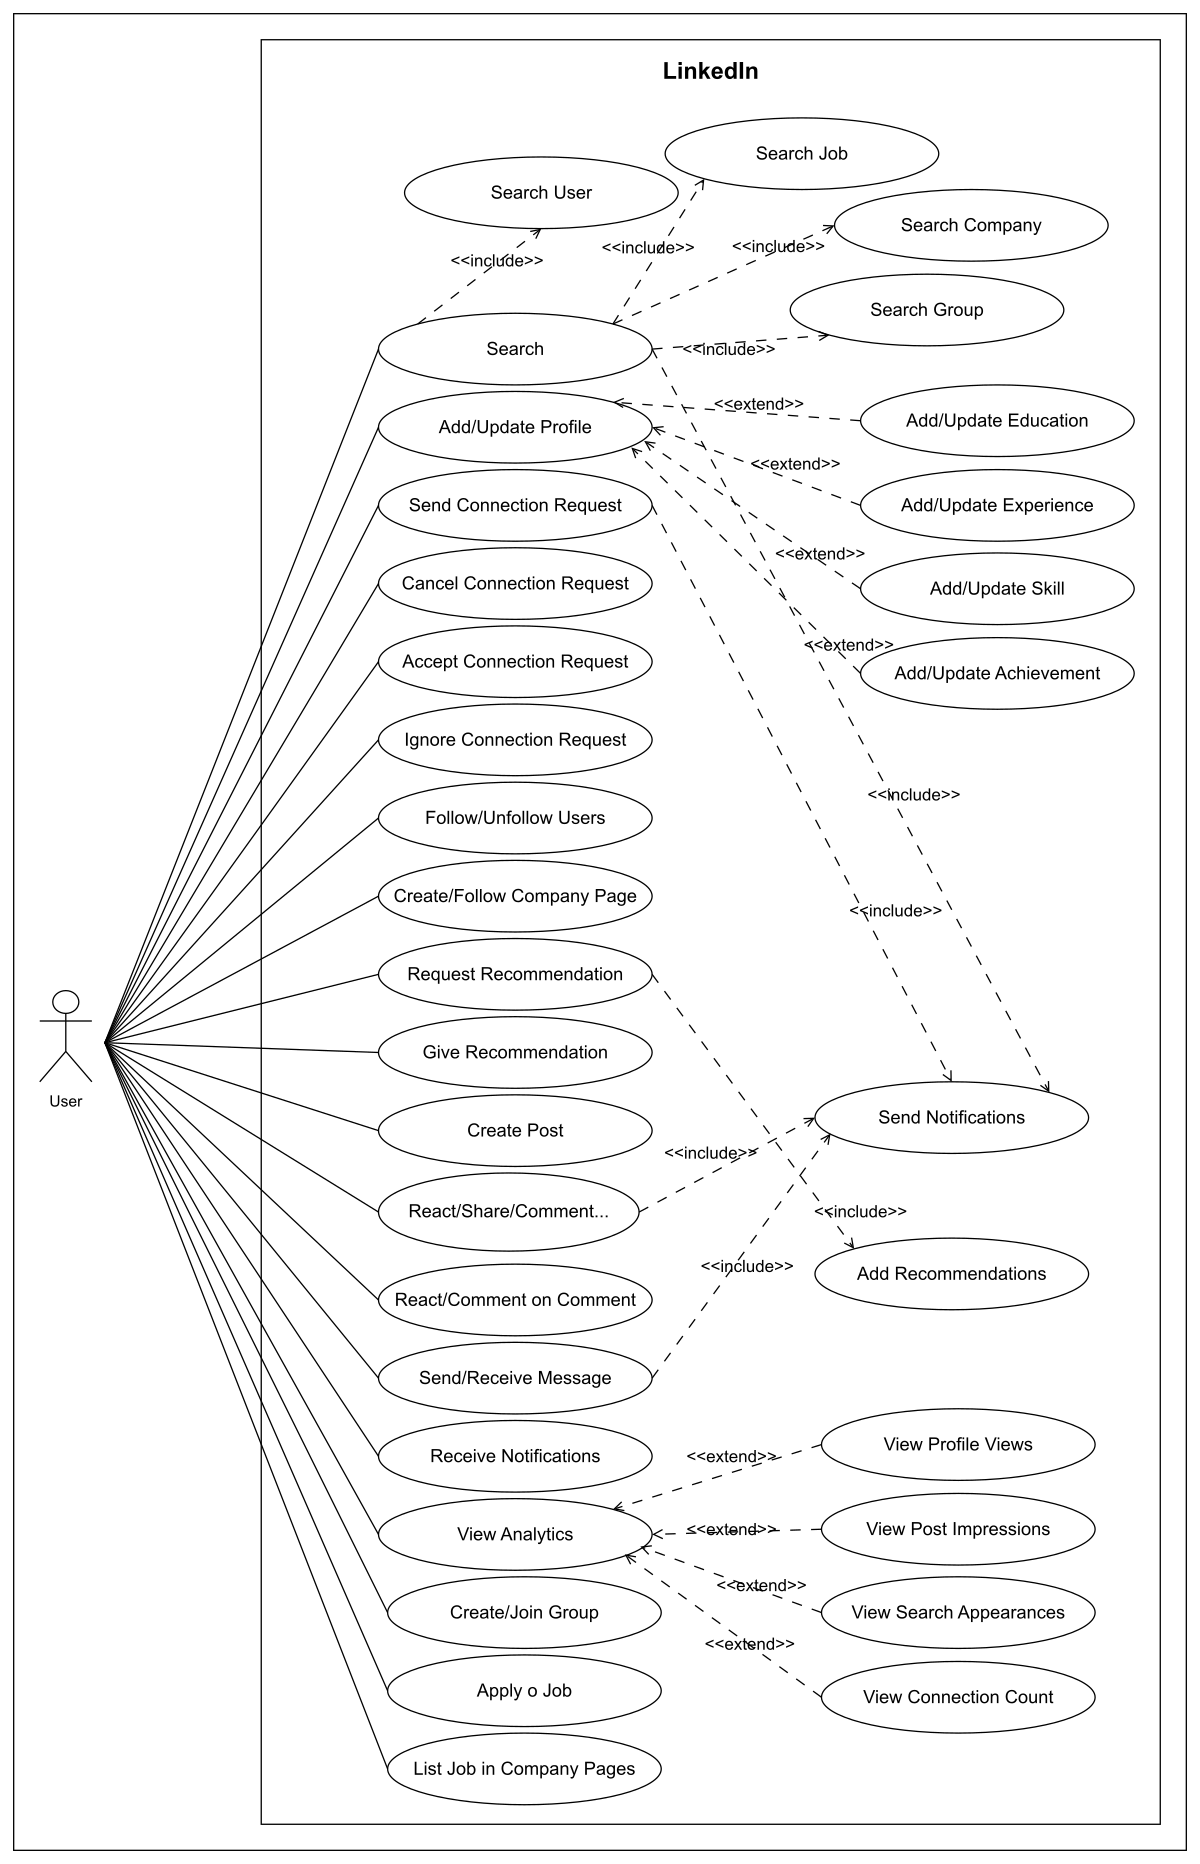
\includegraphics[width=0.5\textwidth]{Images/chapter_27/section_6663591366492160/4699361307918336.png}
 \caption{The use case diagram of LinkedIn}
\end{figure}

In the next lesson, we'll discuss the class diagram with a detailed explanation of all classes and their relationship with each other.

% End of section content